%%%%&latex
\documentclass[hidelinks,10pt]{article}
\usepackage{graphicx}
\usepackage{amsmath}
\usepackage{enumerate}
\usepackage{url}
\usepackage{amsfonts}

\usepackage[linesnumbered,ruled,vlined]{algorithm2e}

\usepackage{listings}
\usepackage{color}
\usepackage{hyperref}

\addtolength{\oddsidemargin}{-.5in}%
\addtolength{\evensidemargin}{-.5in}%
\addtolength{\textwidth}{1in}%
\addtolength{\textheight}{1.3in}%
\addtolength{\topmargin}{-.8in}%

%\pdfminorversion=4
% NOTE: To produce blinded version, replace "0" with "1" below.

\begin{document}

\def\spacingset#1{\renewcommand{\baselinestretch}%
{#1}\small\normalsize} \spacingset{1}

%%%%%%%%%%%%%%%%%%%%%%%%%%%%%%%%%%%%%%%%%%%%%%%%%%%%%%%%%%%%%%%%%%%%%%%%%%%%%%


\title{\bf MountainSort User Guide}
\author{Jeremy F. Magland\hspace{.2cm}\\
  Center for Computational Biology, Simons Foundation\\
  }
\maketitle

\bigskip
\begin{abstract}
This is an overview of the MountainSort software for automated spike sorting and visualization. Our objectives are threefold. The first is to implement an automated spike sorting algorithm requiring minimal user intervention. Second, we provide interactive visualization tools for exploring the output of this and other spike sorting softwares. Finally, we provide an algorithm-independent framework for objectively validating spike sorting performance by reporting a reliability metric for each detected neuron.
\end{abstract}

\tableofcontents

\vfill

\newpage

\section {Introduction}

% Improve the intro
Our objectives are threefold. The first is to implement an automated spike sorting algorithm requiring minimal user intervention. Second, we provide interactive visualization tools for exploring the output of this and other spike sorting softwares. Finally, we provide an algorithm-independent framework for objectively validating spike sorting performance by reporting a reliability metric for each detected neuron.

\subsection {Importance of automation}

Manual human intervention as part of a spike sorting pipeline is problematic for a number of reasons. The workload may not be practical for a single operator since hundreds of large datasets can be acquired over the course of a few days. Operator bias becomes an issue if the task is shared among several users or the sorting methods of a single user drift over time. Assessing reproducibility or sorting reliability is near impossible since the user cannot be asked to supervise processing of the same dataset multiple times in an unbiased manner. Finally, human-supervised processing cannot easily be transferred between labs and is not compatible with objective comparisons between alternative methods. 

With that said, it is not reasonable to expect a single algorithm to work for all datasets. The experimental setup, noise properties, and hardware-specific artifacts vary significantly between laboratories. A certain degree of tweaking of parameters should be expected. Whenever possible, these should be applied during the preprocessing stage rather than at the end of automated sorting.

\section {Processing algorithm}
Here we describe the algorithm we use for sorting. It comprises the following steps:

\begin{itemize}
\item \textbf{Preprocessing} - bandpass filter and prewhitening
\item \textbf{Detection} - per channel event detect via threshold
\item \textbf{Feature Extraction} - per channel principal component feature extraction using time clips from the electrode channel and its neighbors
\item \textbf{Clustering} - per channel clustering using ISO-SPLIT
\item \textbf{Cluster Splitting} - a second pass of clustering using features from all electrodes
\item \textbf{Template Extraction} - compute average template for each cluster
\item \textbf{Consolidation} - remove redundant clusters since the same neuron is usually identified on multiple electrodes
\item \textbf{Fitting} - Select a subset of the events that explain the underlying data
\end{itemize}

\subsection {Preprocessing}

The input to the preprocessing stage is an $M\times N$ array $Y$ of raw data collected over $N$ timepoints and $M$ electrode channels. The output is two $M\times N$ preprocessed arrays, $Y_\texttt{filt}$ and $Y_\texttt{white}$. The first is used for visualization only and the second is used in the subsequent sorting steps. The options are documented in the MATLAB code.

\begin{algorithm}
\DontPrintSemicolon % Some LaTeX compilers require you to use \dontprintsemicolon instead
\KwIn{$Y$ - $M\times N$ array of raw data}
\KwIn{$o_\texttt{filter}$, $o_\texttt{whiten}$, $o_\texttt{filter2}$ - options}
\KwOut{$Y_\texttt{filt}$ - $M\times N$ array of bandpass filtered data}
\KwOut{$Y_\texttt{white}$ - $M\times N$ array of bandpass filtered and whitened data}

$Y_\texttt{filt}\gets\texttt{bandpass}(Y,o_\texttt{filter})$\;
$Y_0\gets\texttt{whiten}(Y_\texttt{filt},o_\texttt{whiten})$\;
$Y_\texttt{white}\gets\texttt{bandpass}(Y_0,o_\texttt{filter2})$\;

\caption{{\sc Preprocess}}
\label{algo:preprocess}
\end{algorithm}

\subsection {Detection}

Events are detected on a per-channel basis. The output is a collection of timepoints (for each channel) where spike events have been detected. The same event will usually be identified on more than one electrode channel, but this redundancy is handled in subsequent steps. Events are identified whenever the absolute voltage exceeds $\tau\cdot \sigma$ where $\tau$ is a threshold parameter (e.g., $\tau=5$) and $\sigma$ is the standard deviation of the signal on a particular channel. However, to avoid detecting the same event more than once, we do not allow two events to occur within a certain number of timepoints $W$ (for example $40$). Specifically, an event occurs at timepoint $t$ and channel $m$ if $$|Y(m,t)|\geq \tau\sigma$$ and 
$$|Y(m,t)|>|Y(m,t^\prime)|\text{ }\forall t^\prime \text{ s.t. } |t-t^\prime|\leq W.$$

\subsection {Feature Extraction}

Principal component features are extracted for each channel separately, using data from the channel and its neighbors. The set of neighboring channels is determined by the geometric electrode layout and is specified by an $M\times M$ adjacency matrix. Time clips of $T$ timepoints centered around each event are extracted, and principal component analysis is applied on resulting set of vectors. The dimension of the vectors is $M_m\cdot T$ where $M_m$ is the number of channels adjacent to channel $m$. The output for each channel is a $P\times E_m$ array of PCA features, where $P$ is the number PCA components (e.g., 3) and $E_m$ is the number of events detected on channel $m$.

\subsection {Clustering}

Clustering is performed on each channel separately by applying the ISO-SPLIT algorithm to the extracted feature vectors. This algorithm is designed to have zero adjustable parameters. For example, unlike $k$-means, the number of clusters does not need to be specified in advance. It is a density-based algorithm that assumes that clusters are unimodal and that any two distinct clusters are separated by a region of relatively lesser density. A statistical test is used at each iteration to determine whether clusters should be merged or redistributed. More details can be found on the arXiv (http://arxiv.org/abs/1508.04841).

The output for each channel $m$ is a list of integer labels between $1$ and $K_m$, one for each event, where $K_m$ is the number of clusters identified by the algorithm.

\subsection {Cluster Splitting}

The clustering stage above only uses data from the neighborhood of each electrode channel. Sometimes this is insufficient to separate clusters that may differ only on channels that are geometrically separated from the primary loading channel. Therefore a second clustering stage is used to test each previously-identified cluster for splitting, using data from all channels. Again, PCA features are extracted and ISO-SPLIT is employed.

\subsection {Template Extraction}

A $M\times T$ template $W_k$ is computed for each cluster $k=1,\dots,K$ identified in the previous steps. This is done by taking the average of time clips of size $T$ extracted at all event timepoints labeled as cluster $k$. Note that at this stage the set of templates will have redundancies since the same neuron will usually be identified on more than on channel.

\subsection {Consolidation}

As mentioned above, the same neuron will usually be identified on more than one channel, and therefore redundancies need to be eliminated. In most cases, each neuron will have a primary electrode on which it loads with greater energy than on any other electrode. Therefore, if cluster $k$ was identified from channel $m_k$ and 
$$\|W_k(m_k,\cdot)\|_2<\mu \|W_k(m^\prime,\cdot)\|_2$$
for some other channel $m^\prime$, then we know that $k$ is a redundant cluster and can therefore be eliminated. Here, $\mu<1$ is a tolerance constant (e.g., $\mu=0.9$). In other words, we eliminate all clusters that whose primary load channel is not the channel used to identify the cluster.

The above heuristic handles most redundancies. However, sometimes a neuron fires with around the same energy on two nearby electrodes. We therefore use a second criterion (in a second pass) to handle these situations. Let $n_{k_1}$ be the number of events classified as type $k_1$ and let $n_{k_1,k_2}$ be the number of these events which are near (within $20$ time points) an event classified as $k_2$. Let $0<\tau_c\leq 1$ be a \emph{coincidence} threshold (e.g., $\tau_c=0.5$). If $n_{k_1,k_2}>\tau_c n_{k_1}$ or $n_{k_1,k_2}>\tau_c n_{k_2}$, then we consider $k_1$ and $k_2$ to represent the same neuron and therefore we eliminate either $k_1$ or $k_2$, whichever occurs with less frequency.

Note that \emph{consolidation} is different from \emph{merging}. Merging denotes taking a union of two sets of events, whereas our consolidation simply involves deleting a cluster. This makes sense because we are handling the situation where two clusters (occurring on different channels) actually represent the same neuron, and one can therefore be deleted.

\subsection {Fitting}

At this point we have a collection of $L$ labeled events $\{(t_j,l_j,m_j)\}_{j=1}^L$, where $t_j$ is the timepoint, $l_j$ is the integer label identifying the spike type, and $m_j$ is the primary channel for this spike type. So far we haven't been trying to \emph{explain} or \emph{fit} the data array, but rather we were just detecting likely events and clustering them based on similarity. Ideally we would like
$$Y_\texttt{white}(m,t)\approx\sum_{j=1}^L W_{l_j}(m,t-t_j),$$
where $W_k$ is the average spike type template as defined above.
But we haven't been using this formulation in any way. In fact, the detections of two events $(t_{j_1},l_{j_1},m_{j_1})$ and $(t_{j_2},l_{j_2},m_{j_2})$ are completely independent when $m_{j_1}\neq m_{j_2}$ even when the timepoints are equal or very close.

In this fitting stage, we use a greedy fitting approach to reduce to a subset of the labeled events that best explain the whitened data. The implementation of the algorithm is a bit tricky, and involves several passes, and efficient storage of various computed quantities. For now I just state the inputs and outputs:

\begin{algorithm}
\DontPrintSemicolon % Some LaTeX compilers require you to use \dontprintsemicolon instead
\KwIn{$Y_\texttt{white}$ - $M\times N$ array of raw data}
\KwIn{S=$\{(t_j,l_j,m_j)\}_{j=1}^L$ - a collection of labeled events}
\KwIn{$\{W_1,\dots,W_K\}$ - spike templates}
\KwOut{$\tilde{S}\subset S$ - a subset of the labeled events that best explain the data}

\caption{{\sc Fit}}
\label{algo:fit}
\end{algorithm}

%If a multi-electrode array is used and the user wishes to provide information about the geometry of the detectors, an $M\times M$ binary adjacency matrix may be supplied to specify the neighbors to each channel.

\section {Processing software}

All processing routines are implemented in C++ and are runnable either as UNIX command line utilities or using one of the MATLAB wrappers provided in the source package. The input and output data are always files, usually in the .mda format (see http://magland.github.io/articles/mda-format/). To make efficient use of RAM, files are processed in chunks whenever possible. In addition, parallel processing via OpenMP is used whenever possible. For these reasons, the source code may be difficult to read, even for basic operations such as threshold-based detection. The documentation of source code will improve over time.

\subsection {The command line program}

All processing commands are applied by running the bin/mountainsort executable. The first command line argument is the name of the processing procedure, or processor. Then the processor-specific options are supplied as additional arguments. For example, detection is applied using the following command:

\lstset{basicstyle=\ttfamily,
  showstringspaces=false,
  commentstyle=\color{red},
  keywordstyle=\color{blue}
}
\begin{lstlisting}[language=bash]
./mountainsort detect --input=in.mda --output=out.mda
  --inner_window_width=40 --outer_window_width=1000
  --threshold=5
\end{lstlisting}

Run the mountainsort program with no arguments to see a list of the available processors, and run it with a single argument to see the version of the processor and a list of available processor-specific options.

\subsection {Automatic non-redundant processing}

The mountainsort command line utility has a built-in provenance tracking capability so that actual computations are only performed the first time a command is run. This allows the user to conveniently rerun scripts without waiting for the entire pipeline. For example, if a parameter in the consolidation stage is modified, then only the processing for the final steps are rerun.

When a mountainsort processor executes, it first checks whether the output files already exist. If they do, then it compares those files with a database of all previous runs (stored in bin/.process\_tracker) to search for a match. Two processing runs match if the input files, input parameters, and output files all match. The processor only runs if no such match is found.

\subsection {MATLAB wrappers}

For convenience, each mountainsort processor may be run using the corresponding MATLAB wrapper. For example, see processing/mscmd\_detect.m. Note that no data arrays are stored in MATLAB memory since all processors operate on files. In this way, automatic provenance tracking and non-redundant processing applies to the MATLAB wrappers as well as the command line utility.

An example processing script that uses the MATLAB wrappers can be found in the example\_mscmd directory. Note that execution is almost instantaneous the second time the script runs.

\section {Visualization software}

The main visualization program is located at mountainview/bin/mountainview. This is an interactive visualization tool only and does not run any processing routines. The idea is that the same viewer may also be used to view the output of third party spike sorting software. An example call to this program via MATLAB can be found at example\_mscmd/example\_mscmd\_view.m.

\subsection {Main window}

A screenshot of the main MountainView window is shown in Fig. \ref{fig:mountainview_main_window}.
The upper-left window lists the identified neurons with some statistics. This list may be sorted by any of the columns by clicking on the relevant column header. The center-left window contains a graphical view of the firing rates for the various neurons. The x-axis is time and the y-axis is the cumulative number of events. Each curve represents a different neuron. The lower-left window shows the geometric layout of the electrodes. The colors correspond to the currently selected neuron and show the maximum or minimum voltages over the duration of the template waveform. Note that this plot is most relevant when viewing non-whitened data.

The upper-right view shows the template waveforms for the identified neurons. Each column is a different neuron, and the rows correspond to the different electrode channels. The center-right view shows auto-correlograms. These are histograms depicting the time differences between pairs of firing of the same neuron. Ideally, each auto-correlogram will have a dip at the center which is explained by physiologic refractory-period constraints. The lower-right window shows the preprocessed raw data. Zooming in on this view reveals the labels as vertical red bars.

\begin{figure}[!h]
\centering
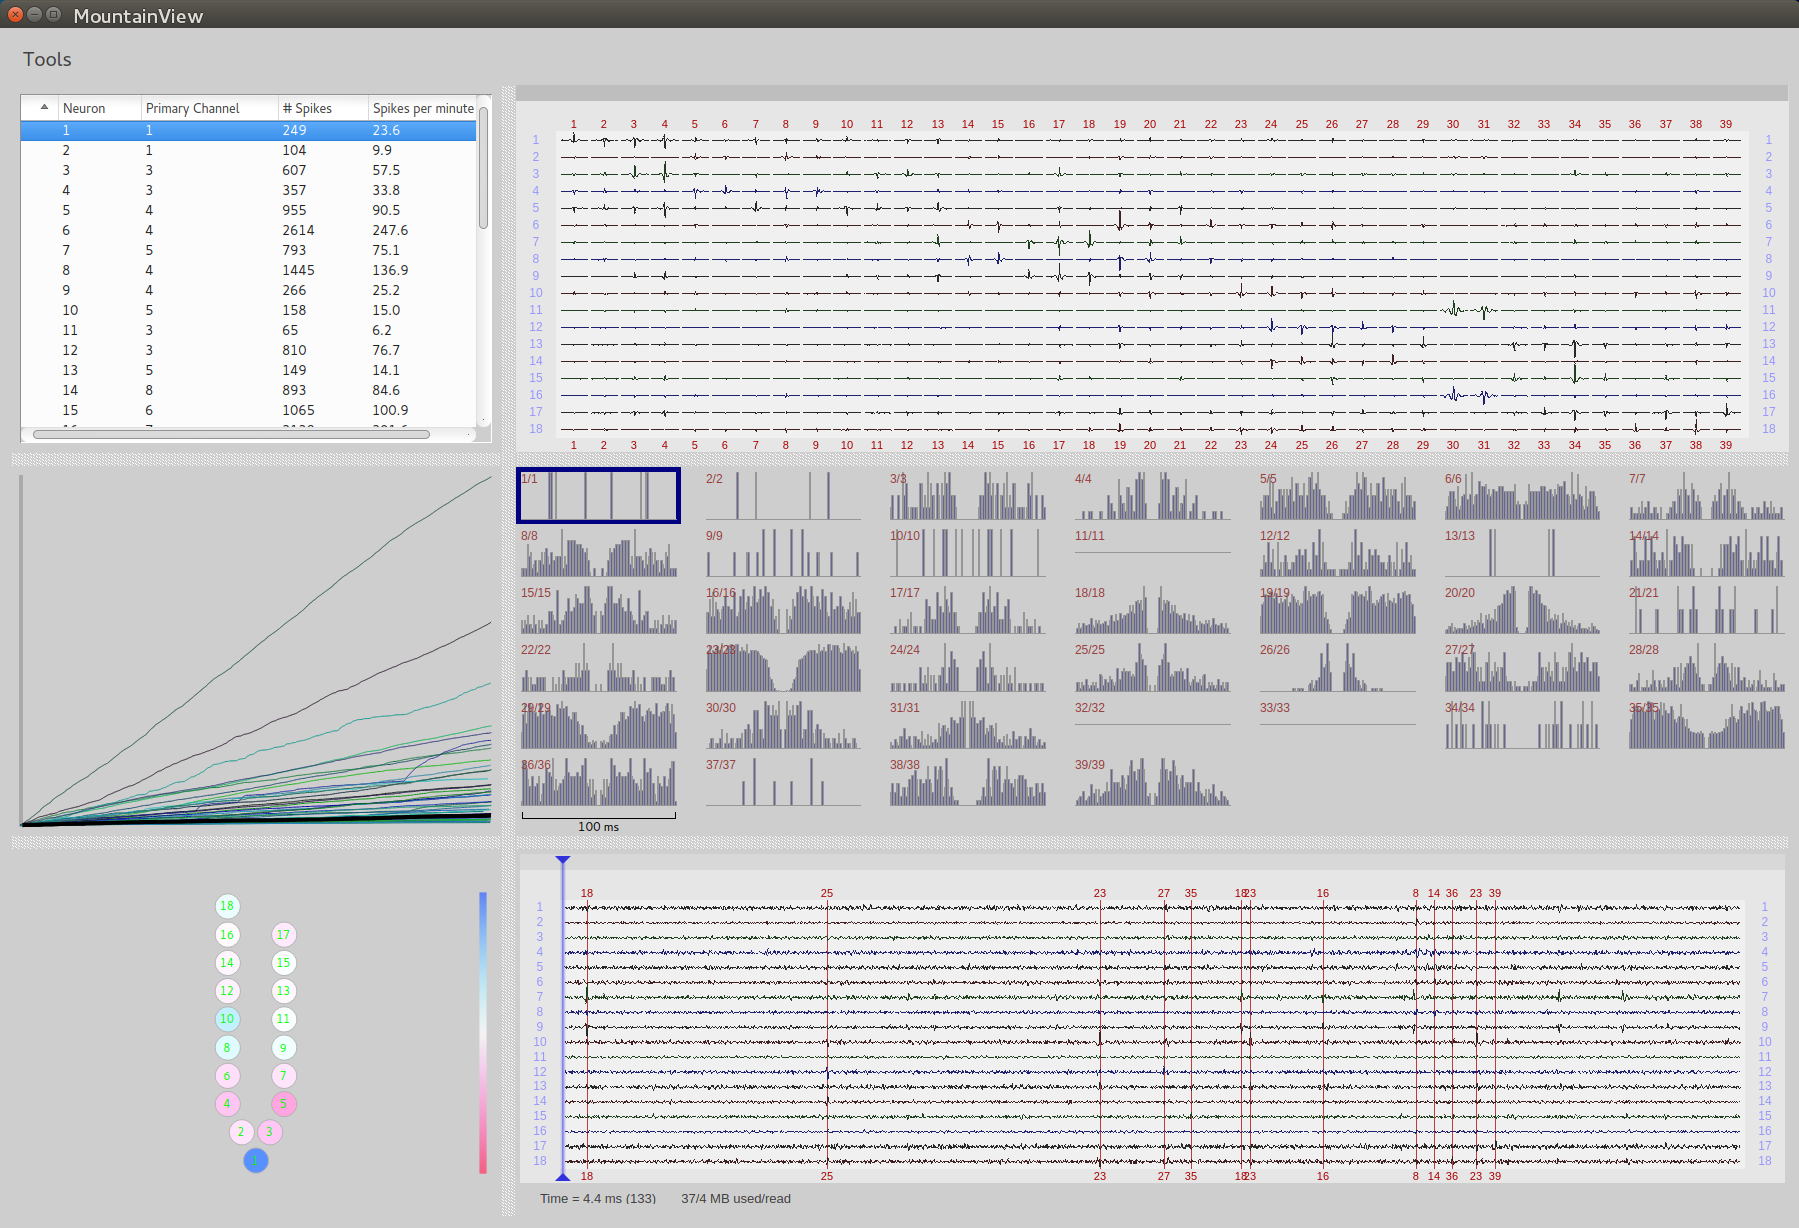
\includegraphics[width=6in]{images/mountainview_main_window.png}
\caption{
MountainView main window.
}
\label{fig:mountainview_main_window}
\end{figure}

\subsection {Individual neuron window}

A detailed view of the behavior of an individual neuron can be seen by double-clicking on one of the auto-correlograms in the main window (or by using the option in the Tools menu). See Fig. \ref{fig:mountainview_neuron_window}.

The upper-left pane shows the template, or average waveform, for this neuron. The bottom-left pain shows a 3D-rotatable view of the first 3 principal components for all detected events associated with this neuron. The upper-right window shows all of the extracted clips. This view can be rapidly zoomed in and out to get a feel for the homogeneity of the event clips. The center-right window shows the cross-correlograms between the selected neuron and all other neurons. These histograms show the distribution of time differences between pairs of events. Ideally, these histograms should all be flat, except for the one that corresponds to an auto-correlogram, as above. The lower-right window is the raw data view with only the selected neuron labeled.

\begin{figure}[!h]
\centering
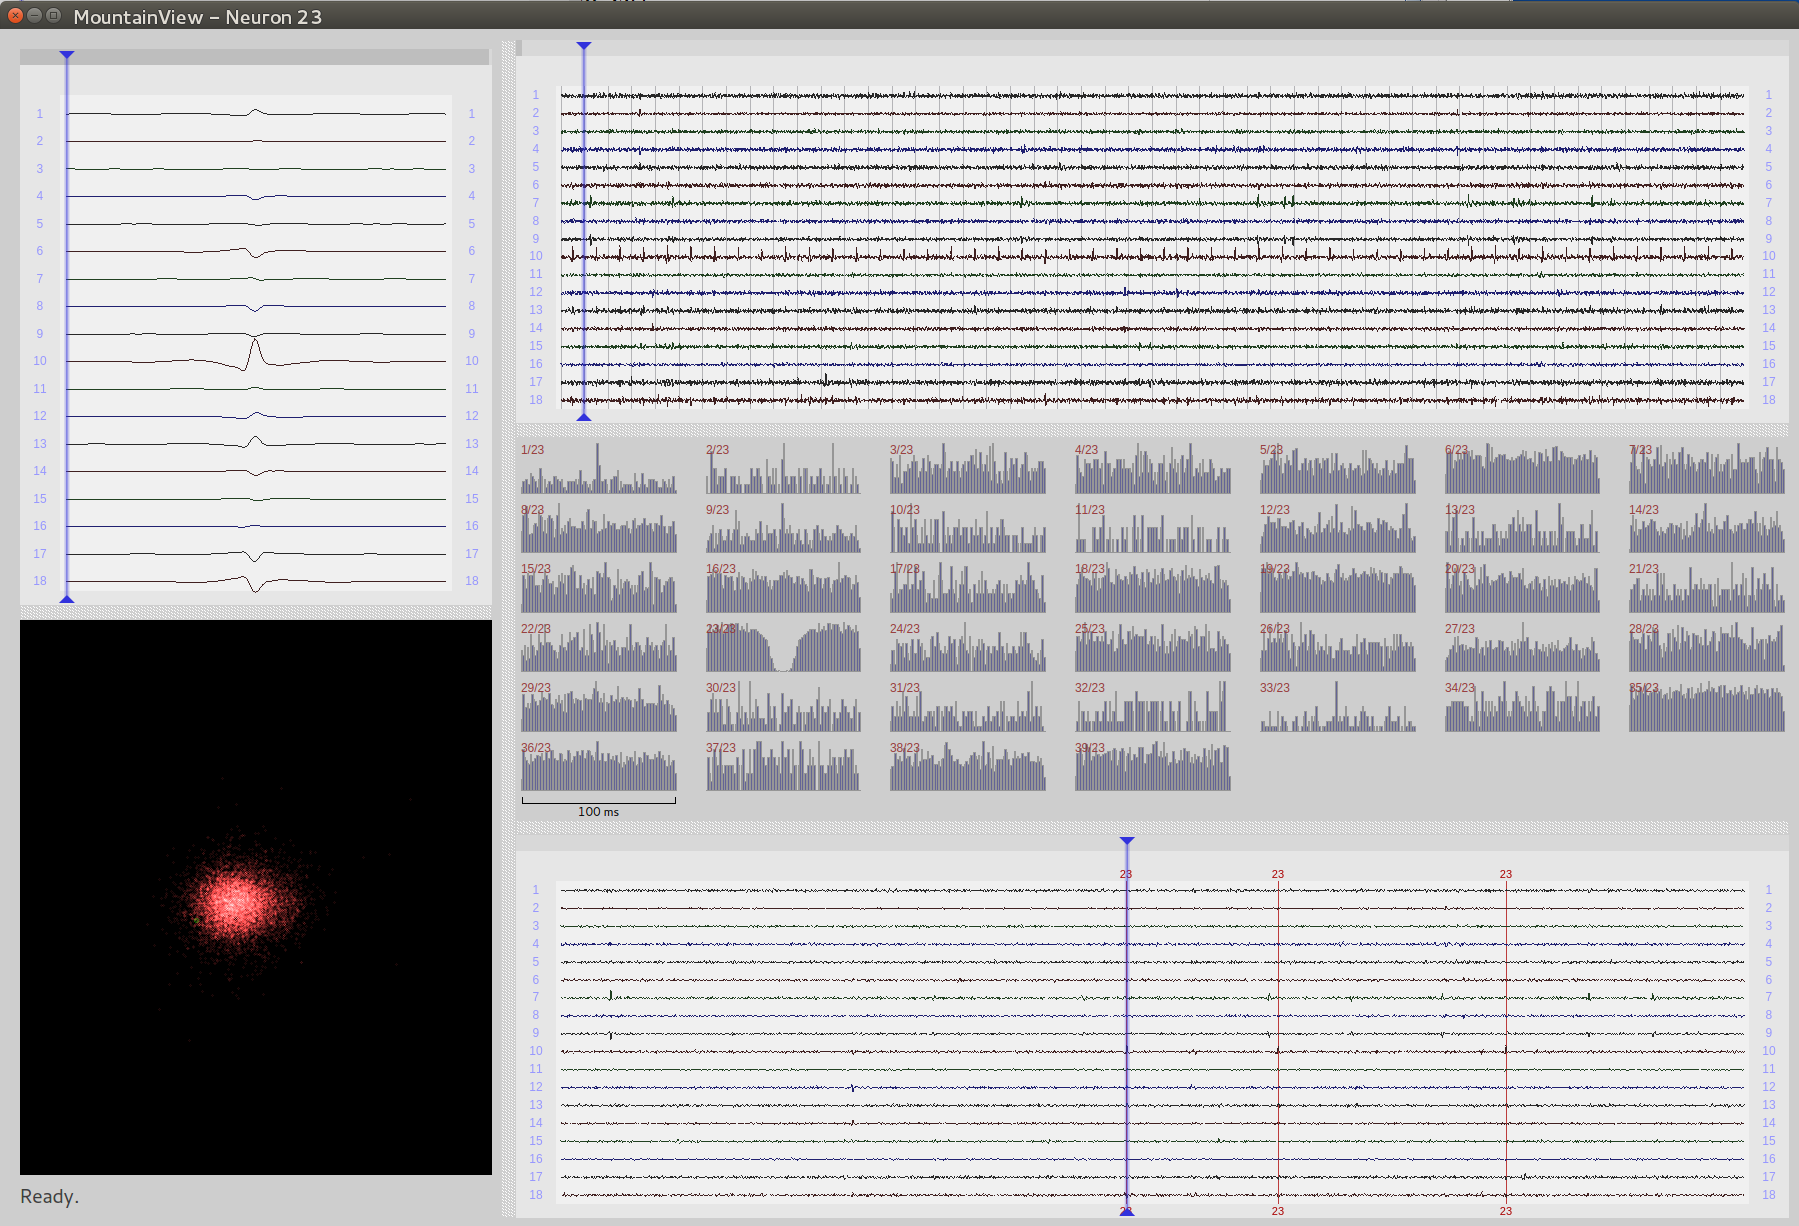
\includegraphics[width=6in]{images/mountainview_neuron_window.png}
\caption{
Individual neuron window.
}
\label{fig:mountainview_neuron_window}
\end{figure}

\subsection {Neuron comparison window}

A comparison of two or more neurons is available by selecting the corresponding auto-correlograms in the main window (using the Ctrl Key) and then selecting Tools->Compare Neurons from the menu. See Fig. \ref{fig:mountainview_compare_window}.

The upper-left pane shows the template waveforms of the selected neurons. The lower-left pane is a 3D-rotatable view of the first tree principal components for the events of the selected neurons. Each neuron is given a different color. The center-right window is the matrix of cross-correlograms. Ideally, the diagonal histograms will have refractory period dips. The lower-right view shows the raw data with only the selected neurons labeled.

\begin{figure}[!h]
\centering
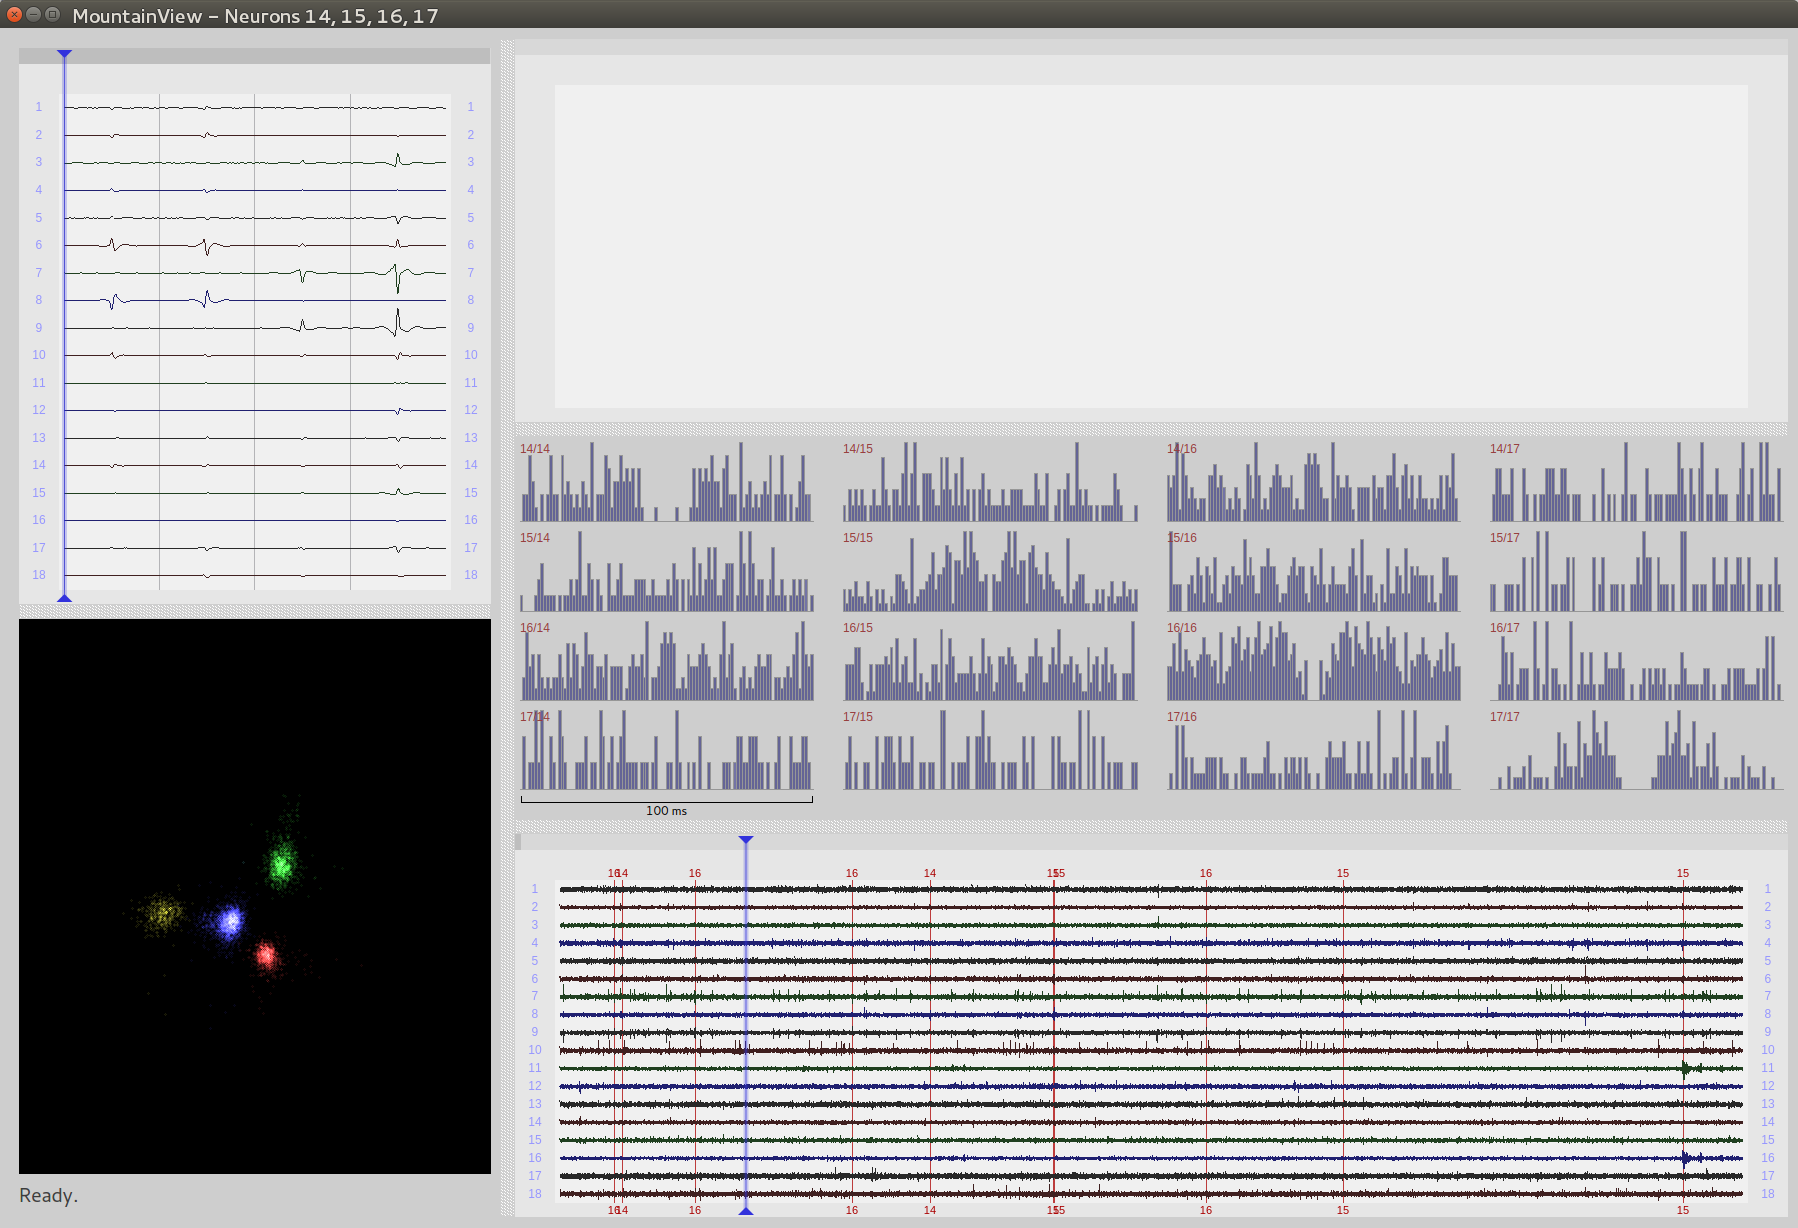
\includegraphics[width=6in]{images/mountainview_compare_window.png}
\caption{
Neuron comparison window.
}
\label{fig:mountainview_compare_window}
\end{figure}



\section {Installation}

The core MountainSort software is written in Qt5/C++. It requires Qt5 development environment to be installed on your system. For now MountainSort runs on Linux. It should work on Mac without too much trouble. Windows is a pain.

See the README.txt file for detailed instructions.


\end{document}
